% Gemini theme
% https://github.com/anishathalye/gemini

\documentclass[final]{beamer}

% ====================
% Packages
% ====================

\usepackage[T1]{fontenc}
\usepackage{lmodern}
\usepackage[size=custom,width=106.68,height=60.96,scale=0.85]{beamerposter}
\usetheme{custom}
\usecolortheme{tntech}
\usepackage{graphicx}
\usepackage{booktabs}
\usepackage{tikz}
\usepackage{pgfplots}
\usepackage{pgf}
\usepackage{multicol}
\usepackage{mathtools}

% ====================
% Lengths
% ====================

% If you have N columns, choose \sepwidth and \colwidth such that
% (N+1)*\sepwidth + N*\colwidth = \paperwidth
\newlength{\sepwidth}
\newlength{\colwidth}
\setlength{\sepwidth}{0.025\paperwidth}
\setlength{\colwidth}{0.3\paperwidth}

\newcommand{\separatorcolumn}{\begin{column}{\sepwidth}\end{column}}

\newcommand{\minus}{\scalebox{0.75}[1.0]{$-$}}
\newcommand{\smallequals}{\scalebox{0.75}[1.0]{$=$}}
\newcommand{\sectionHeading}[1]{\vskip2.0ex \textbf{#1} \vskip0.25ex}

% ====================
% Title
% ====================

\logotitle{
\includegraphics[height=5.0cm]{tntechgold.png}}
\title{Biologically Extending the Gen 2 Artificial Neural Network}
\author{Jesse Roberts \inst{1} \and Dr. Douglas Talbert \inst{2}}
\institute[shortinst]{\inst{1} Vanderbilt University \samelineand \inst{2} Tennessee Technological University}

% ====================
% Body
% ====================
\pgfplotsset{compat=1.16}
\begin{document}

\begin{frame}[t]
\begin{columns}[t]
\separatorcolumn

\begin{column}{\colwidth}

  \begin{block}{Biological Neurons}

    \begin{figure}
      \centering
      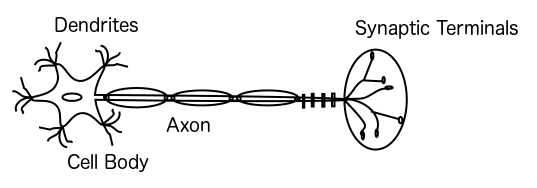
\includegraphics[width=20.0cm]{Neuron.png}
      \caption{Neuron Diagram}
    \end{figure}

    \begin{itemize}
      \item \textbf{Dendrites} provide the input field to the neuron
      \item The voltage difference from \textbf{cell body} to the exterior of the cell controls action potential
      \item The \textbf{axon} carries the action potential to other locations in the network
      \item \textbf{Synaptic terminals} transmit the action potential from the axon to other neural dendrites

    \end{itemize}

    With the arrival of each \textbf{action potential} at a \textbf{synaptic terminal}, \textbf{neurotransmitters} are released and carried \textbf{into the neuron} by way of \textbf{ion channels and pumps}. The ions \textbf{change the voltage} present across the \textbf{membrane of the cell body}. If the membrane voltage increases \textbf{past the action potential threshold}, an \textbf{action potential} will occur and \textbf{propagate along the axon} to the \textbf{synaptic terminals}. A membrane voltage that has been elevated is referred to as \textbf{depolarized}. In homeostasis a neuron attempts to enforce \textbf{polarization}, remaining ready to receive input leading to an action potential. 

    \begin{equation}
      \label{Formula:Neuron1}
      r_{action} = \minus r_{pol} + \sum  \alpha * r_{depol}, \quad \alpha \geq 0
    \end{equation}

    \begin{itemize}
      \item \textbf{firing rate} of the target neuron is \textbf{dependent} upon the \textbf{rate of depolarization}
      \item $\boldsymbol r_{pol}$ is the internal \textbf{rate of polarization}
      \item $\boldsymbol r_{depol}$ is the \textbf{rate} at which a specific \textbf{synapse is firing}
      \item $\boldsymbol \alpha$ is the amount of \textbf{neurotransmitter released} with each pulse at the synaptic terminal
      \item $\boldsymbol r_{action}$ is the \textbf{rate of action potential} propagated along the axon
      \item Summation accounts for multiple synapses
    \end{itemize}

  \end{block}

  \begin{block}{Biological Interneurons}

    Interneurons provide external polarization to the biological neural network. Eq \ref{Formula:Neuron1} is modified to reflect external polarization in \ref{Formula:Neuron1Interneuron}.

    \begin{equation}
      \label{Formula:Neuron1Interneuron}
      r_{action} = \minus r_{pol} + \sum  \alpha *\beta_{Inter}* r_{depol}, \quad 0 \leq \beta \leq 1 \quad \alpha \geq 0
    \end{equation}

    \begin{itemize}
      \item \textbf{Interneurons} allow for \textbf{selective gating} of inputs to different regions of the dendrite
      \item \textbf{Interneurons} facilitate \textbf{dynamic changes} in the \textbf{relative contribution} of inputs
      \item $\boldsymbol \beta_{Inter}$ accounts for the gating associated with a particular synaptic connection
    \end{itemize}
    
    \vskip3ex
    
    \footnotesize{*Neither Eq \ref{Formula:Neuron1} or \ref{Formula:Neuron1Interneuron} is intended to be complete characterizations of a neuron. Rather both should be understood to capture the relevant pieces of neural activity necessary to develop Gen 1 and 2 neural networks.}

  \end{block}

\end{column}

\separatorcolumn

\begin{column}{\colwidth}

  \begin{block}{Artificial Neurons}

    \textbf{Gen 1 ANNs} are considered those limited to classification. They are incapable of performing regression because the output assumes only the \textbf{values one or zero}. The perceptron is such a model. This model characterizes \textbf{neurons as switches} as shown in Eq \ref{Formula:Gen1ANN}.


    \begin{equation}
      \label{Formula:Gen1ANN}
      net = \begin{cases} 
        0 & b + \sum w_{j}*I_{j} \geq 0 \\
        1 & b + \sum w_{j}*I_{j} < 0
        \end{cases}
    \end{equation}

    \begin{itemize}
      \item $\boldsymbol w_{j}$ represents the relative amount of neurotransmitters released or, $\alpha$ in Eq \ref{Formula:Neuron1}
      \item $\boldsymbol I_{j}$ is the firing rate present at the $j^{th}$ synapse 
      \item $\boldsymbol b$ is the bias associated with this neuron or, $r_{pol}$ in Eq \ref{Formula:Neuron1}
    \end{itemize}

    \textbf{Gen 2 ANNs} are where the bulk of research in computer science has been focused. The ability to output a \textbf{continuous value from zero to one} provided the ability to \textbf{learn non-linear regressive approximations} thanks to \textbf{continuously differentiable activation functions}. The typical equation for a Gen 2 ANN is presented in Eq \ref{Formula:Gen2ANN}. The step function has been replaced by the \textbf{sigmoid function} represented by $\boldsymbol \sigma$. 

    \begin{equation}
      \label{Formula:Gen2ANN}
      net = \sigma \left( b + \sum w_{j}*I_{j} \right)
    \end{equation}

    % \begin{columns}[t]
    %   \begin{column}{0.4\colwidth}

    %     \begin{table}[ht]
    %       % increase table row spacing, adjust to taste
    %       \caption{Gen 1 ANN Model Assumptions}
    %       \label{Table:Gen1ANNAssumptions}
    %       \centering
    %       % Some packages, such as MDW tools, offer better commands for making tables
    %       % than the plain LaTeX2e tabular which is used here.
    %       \resizebox{\columnwidth}{!}{%
    %       \begin{tabular}{ c l }
    %         \toprule
    %         \textbf{Number} & \textbf{Assumption}\\
    %         \midrule
    %         1 & Firing Frequency Encoding\\

    %         2 & Steady State\\

    %         3 & Unity Static Firing Rate\\

    %         4 & Learned Inhibition\\

    %         5 & Unconditional Weighting\\
    %        \bottomrule
    %       \end{tabular}}
    %     \end{table}
    %   \end{column}

    %   \begin{column}{0.4\colwidth}
    %     \begin{table}[ht]
    %       % increase table row spacing, adjust to taste
    %       \caption{Gen 2 ANN Model Assumptions}
    %       \label{Table:Gen2ANNAssumptions}
    %       \centering
    %       % Some packages, such as MDW tools, offer better commands for making tables
    %       % than the plain LaTeX2e tabular which is used here.
    %       \resizebox{\columnwidth}{!}{%
    %       \begin{tabular}{ c l }
    %         \toprule
    %         \textbf{Number} & \textbf{Assumption}\\
    %         \midrule
    %         1 & Firing Frequency Encoding\\

    %         2 & Steady State\\

    %         3 & Learned Inhibition\\

    %         4 & Unconditional Weighting\\
    %         & \\
    %         \bottomrule
    %       \end{tabular}}
    %     \end{table}
    %   \end{column}

    % \end{columns}

  \end{block}

\vskip-1em
  \begin{alertblock}{Artificial Interneurons \hskip0.5ex (INNs)}

    \textbf{Contribution}

    \begin{itemize}
      \item \textbf{Extended} the Gen 2 ANN model to include interneurons
      \item \textbf{Facilitated} selectively gating the input along any edge to edge connection between neurons 
      \item \textbf{Derived} the backpropagation equations necessary for an arbitrary INN
      \item \textbf{Outperformed} the base ANN when applied to the MNIST dataset 
    \end{itemize}

    \sectionHeading{INN Model Requirements}

    Given a set $\boldsymbol I$ of inputs to neuron $\boldsymbol n$ it is required that any $\boldsymbol I^{\prime} \in I$ be modifiable such that the set $\boldsymbol I^{\prime} \boldsymbol \Delta \boldsymbol I$ is left unchanged. This lends itself to the addition of some weight $\boldsymbol \beta$ to the ANN equation. $\boldsymbol \beta$ must be variable depending on the inputs presented to the ANN.

    \sectionHeading{INN Model}

    \begin{columns}[t] 

    \centering
    \begin{column}{0.45\columnwidth}
    \begin{figure}
      \centering
      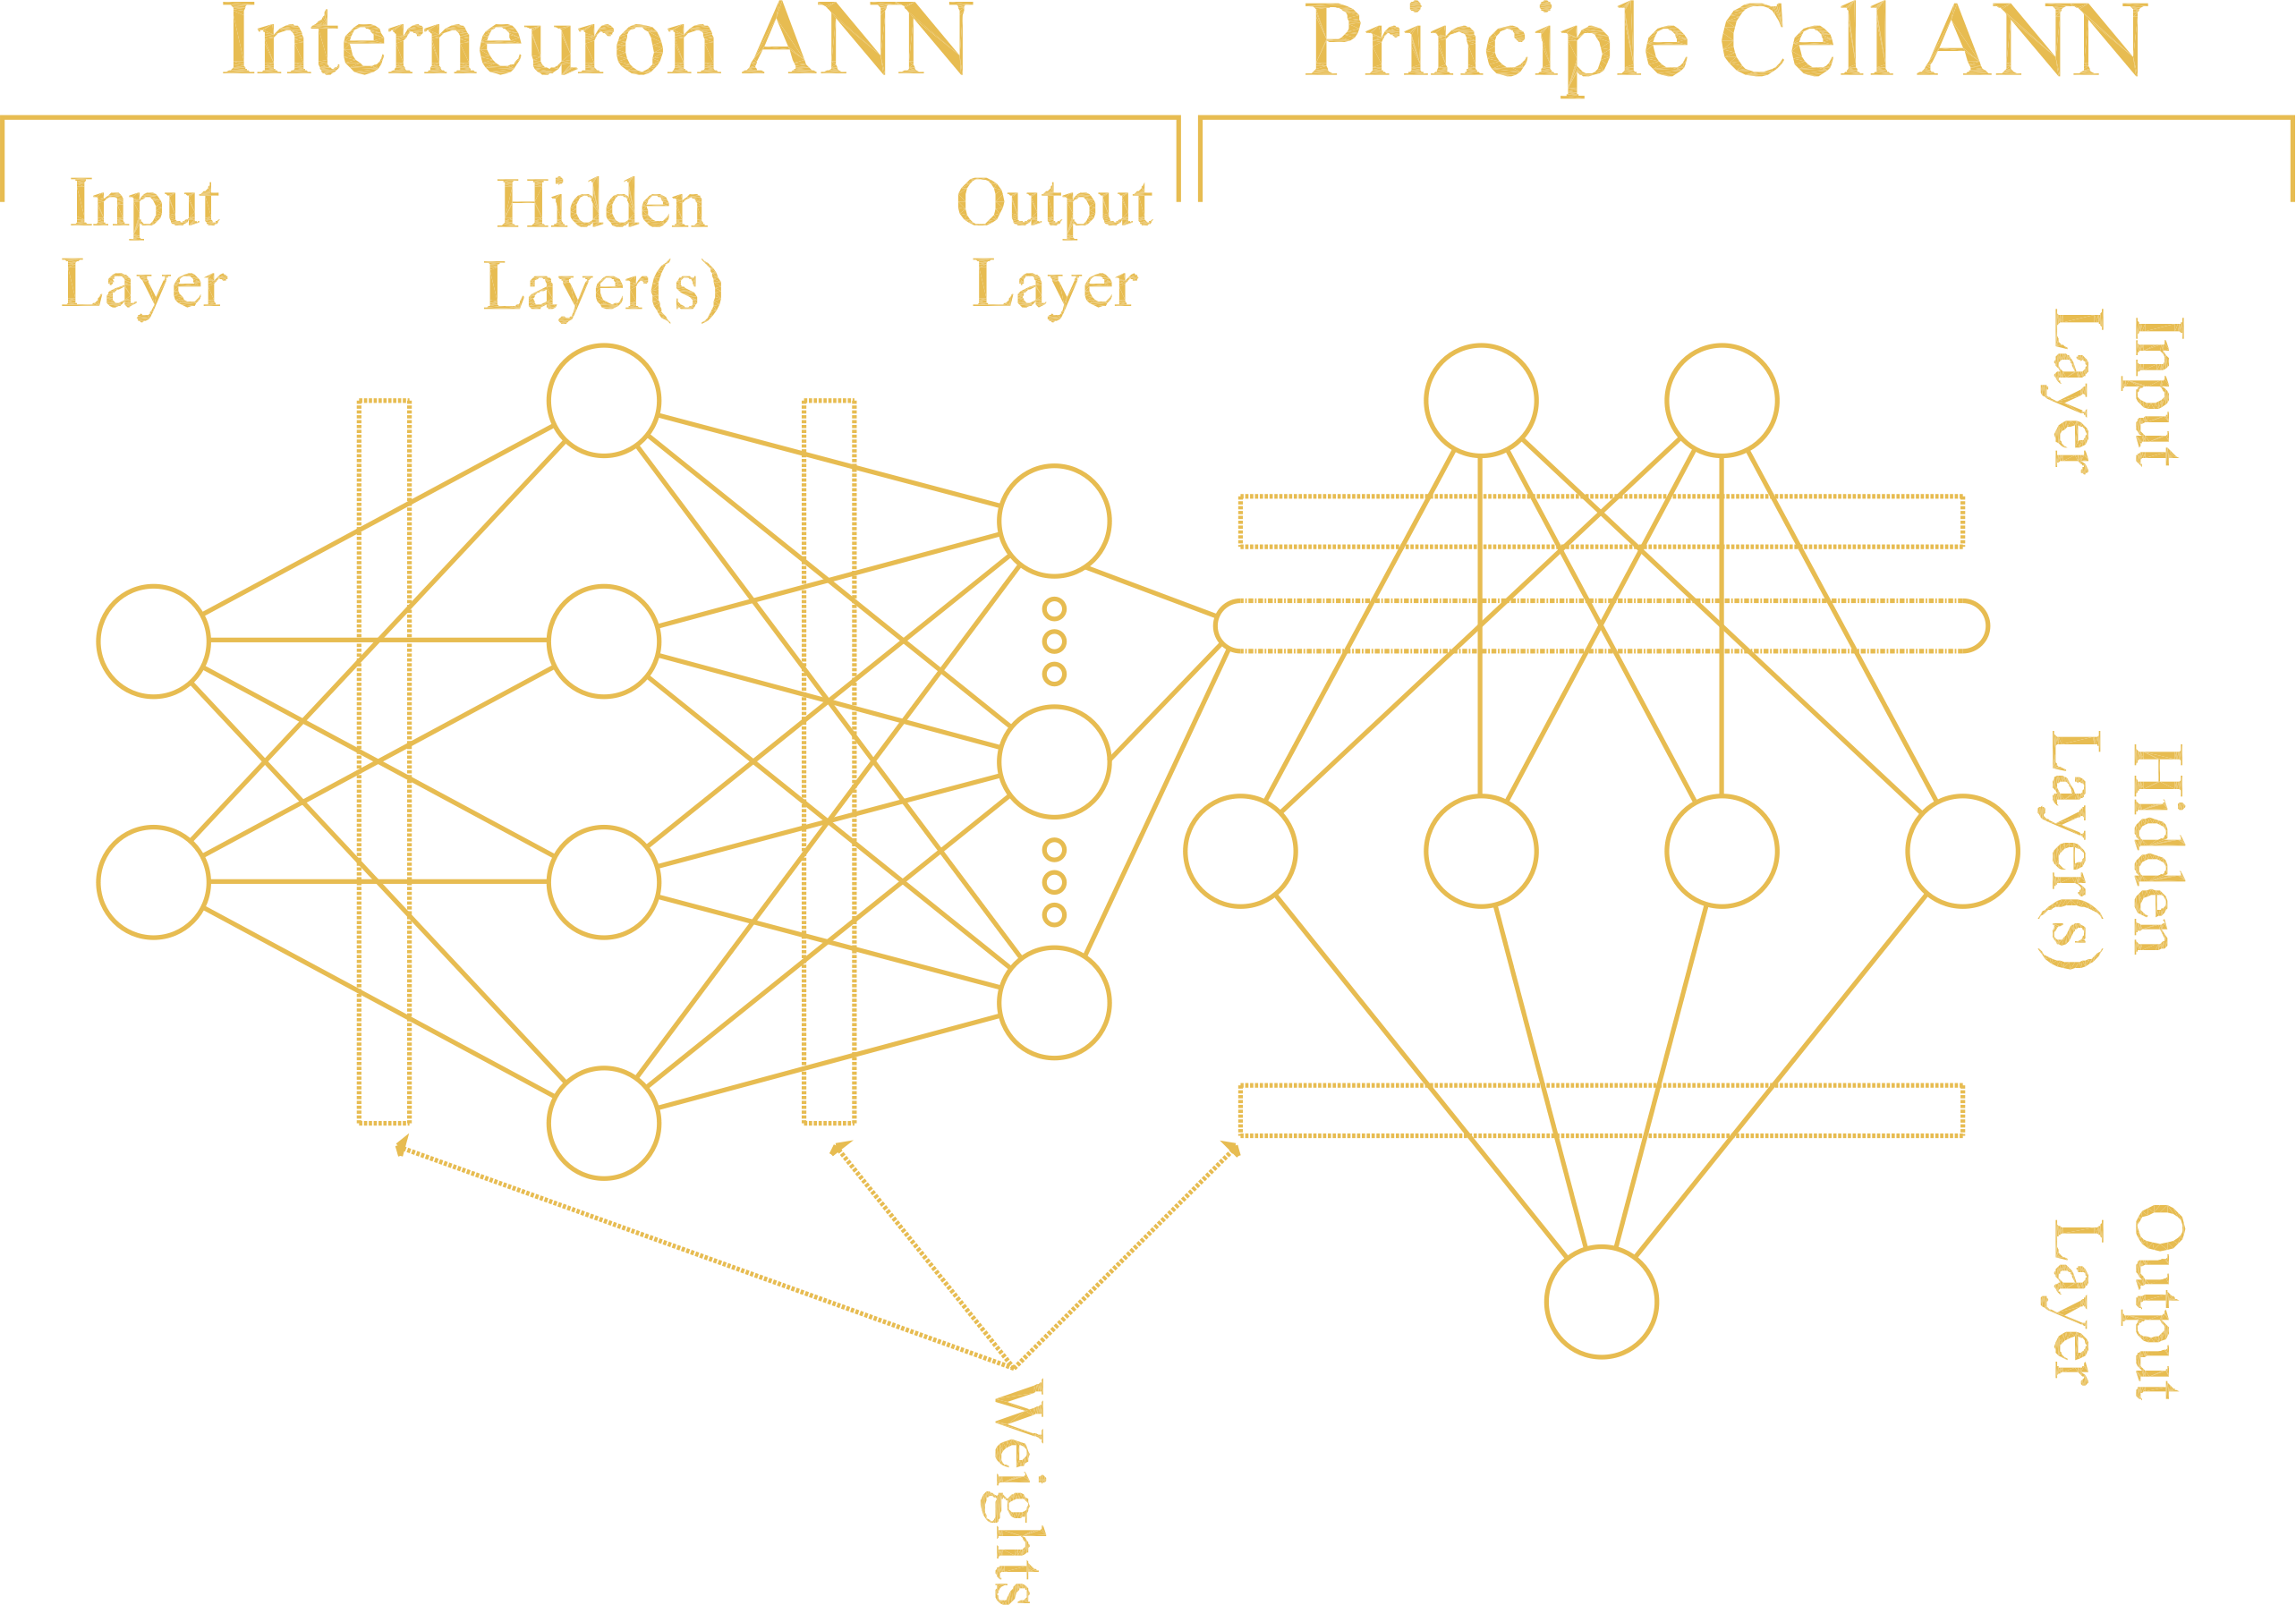
\includegraphics[height=11.0cm]{INN_Topology.png}
      \caption{Neuron Diagram}
    \end{figure}
    \end{column}

    \begin{column}{0.45\columnwidth}

    \vskip3.5ex
    \begin{equation}
      \label{Formula:ANNwInter}
      net = \sigma \left( b + \sum w_{j}*\beta_{j}*I_{j} \right)
    \end{equation}

    \begin{equation}
      \label{Formula:INN}
      \beta_{j} = \sigma \left( b^{\prime} + \sum w^{\prime}_{j}*I^{\prime}_{j} \right)
    \end{equation}
    \end{column}

    \end{columns}


    \vskip0.5ex
    \footnotesize{*It should be understood that the point of this paper is not to build a better performing ANN. It is the beginning of investigation towards a new more biologically plausible model.}

  \end{alertblock}

\end{column}

\separatorcolumn

\begin{column}{\colwidth}


  \begin{block}{Results: Applying an INN to MNIST}

    \sectionHeading{Experimental Setup}

    \begin{itemize} 
      \item \textbf{MNIST} is a well known problem in machine learning
      \item MNIST Consists of 60000 training images of handwritten digits and 10000 test images
      \item The experiment proves the model \textbf{learns and converges} to a solution in a multi-output, large input environment
      \item The INN model was implemented in \textbf{Tensorflow}
      \item Interneurons were only applied to the hidden layer
      \item All other values for the interneuron ANN were the same as the principal cell ANN
      \item The principal cell ANN and interneuron ANN were optimized simultaneously using backpropogation
    \end{itemize}

    \sectionHeading{Experimental Results}

    \begin{itemize} 
      \item The INN \textbf{outperformed} the ANN
      \item The performance of the ANN as applied to the test set was $96.9$
      \item The performance of the \textbf{INN} was $97.2$
      \item The model has been shown to \textbf{converge and perform} better than the naive case
      \item The INN did not outperform the ANN \textbf{more} most likely due to the problem domain
      \item The power fo the INN is believed to be the abilit to \textbf{dynamically contextualize}
    \end{itemize}


  \end{block}

  \begin{block}{Future Work}

    \sectionHeading{Neuroscience}

    Neuroscience has not been able to make a definitive assertion about \textbf{interneuron input feature selection}, we intend to provide an \textbf{answer using this model}. We have chosen a Gen 2 framework because more is computationally known in this domain. The hope is that through the isolation of variables an answer will be approximated.

    \sectionHeading{Multi-Task and Transfer Learning}

    The literature review was rich with similar work in \textbf{multi-task learning}. It is hoped that by training the principal ANN weights with unity interneuron ANN weights, the special case of INN backpropagation, the principal cell ANN will converge to task 1 and allow the interneuron ANN to \textbf{learn task differentiation}. A similar idea can be applied to experiment with \textbf{transfer learning}.

  \end{block}

  \begin{block}{References}

    \begin{multicols}{2}
      \nocite{*}
      \scriptsize{\bibliographystyle{abbrv}\bibliography{poster}}
    \end{multicols}

  \end{block}

\end{column}

\separatorcolumn
\end{columns}
\end{frame}

\end{document}
